%*****************************************
\chapter{Theory and Alternatives}\label{ch:theory_and_alternatives}
%*****************************************

\section{Two Popular Approaches to Modelling Intelligence}

Recently, there have been two directions of research with the goal of
building a machine that explains intelligent human behavior.  The
first approach is to build a baby-machine that learns from scratch to
accomplish goals through interactions with its environment.  The
second approach is to give the machine an abundance of knowledge that
represents correct behavior.

Each of these solutions has benefits and drawbacks.  The baby-machine
approach is good for dealing with novel problems, but these problems
are necessarily simple because complex problems require a lot of
background knowledge.  The data abundance approach deals well with
complicated problems requiring a lot of background knowledge, but
fails to adapt to changing environments, for which the algorithm has
not already been trained.

\section{Adaptability in Complex Environments}

\begin{figure}[bth]
  \center
  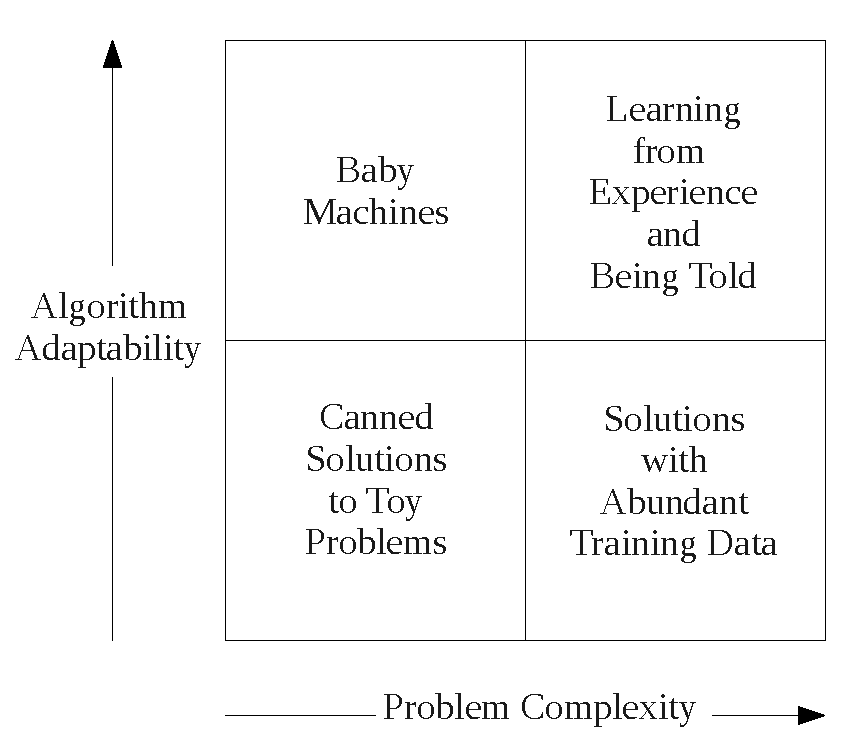
\includegraphics[height=6cm]{gfx/problem_complexity_versus_algorithm_adaptability}
  \caption[Problem complexity versus algorithm adaptability]{Problem
    complexity versus algorithm adaptability.}
  \label{fig:problem_complexity_versus_algorithm_adaptability}
\end{figure}

We would like to build intelligent machines that are able to perform
household tasks, such as cooking, cleaning, and doing the laundry, but
these tasks seem insurmountably complex, containing organically
unpredictable events.  We would like our machines to expertly handle
these extremely complicated problems, and we would also like them to
adapt to learn in unexpected or novel situations.  One popular
approach to building a machine that performs complicated tasks is to
give the machine a large training dataset that details every possible
situation that the machine may find itself within, along with the
correct action in that situation.  This is the so-called
``supervised'' learning approach.  These algorithms do not adapt to
novel situations well, and collecting these datasets is often
impossible for many problems, such as cooking and cleaning because it
is too difficult to enumerate all possible situations, in which the
machine may find itself.  Also, if the machine is cooking a meal, we
would like to be able to explain an idea for a new recipe to the
machine, or to perhaps be a partner in discovering new recipes, or we
may simply want to explain to the machine that a guest has a specific
allergy to walnuts, making that ingredient an exception for this meal
but not others.
Figure~\ref{fig:problem_complexity_versus_algorithm_adaptability}
shows how problem complexity and algorithm adaptability can be thought
of as a two-dimensional space into which different algorithmic
approaches can be used as solutions.

\section{The Abundant Data Approach}

There have been many approaches to modelling complex forms of
reasoning by collecting large amounts of knowledge that describes
correct or acceptable behavior in a domain.  For example, there are
examples of complex multi-agent commonsense simulation environments
collects thousands of examples of users interacting in a complicated
object-oriented social simulation \citep{orkin:2009},
\citep{orkin:2010}.  These systems have complicated domains, but these
projects do not attempt to build agents that attempt to accomplish
goals.  Instead, these systems are inference systems that simply try
to reproduce typical behavior, rather than goal-directed behavior.

There are many commonsense reasoning systems that do not interact with
simulation environments at all, but which attempt to demonstrate
commonsense reasoning by being told large amounts of knowledge.  The
Cyc project is one large such project that has been told large amounts
of logical knowledge \citep{lenat:1990}.  There is also effort
directed toward populating Cyc with knowledge automatically gathered
from the web \citep{matuszek:2005}.  The OpenMind project
\citep{singh:2002} is a project that gathers large amounts of
approximately correct commonsense knowledge from people online.  The
OpenMind knowledge has been turned into many inference systems that
can compare and generate new commonsense knowledge \citep{liu:2004a,
  liu:2004b, speer:2008}.

\section{The Common Sense Reasoning Problem Domain}

Common sense is the set of common reasoning abilities shared by most
people in a given social group.  Another way to say this is that
common sense is the set of reasoning abilities that one would assume
of a typical person that they meet for the first time and know nothing
about.  For example, most people have a naive theory of physics, so
you would expect someone to know that things fall when they are not
supported and liquids flow or are absorbed unless they are in a
container.  Common sense relies on a lot of knowledge that is assumed
that most everyone knows.

%TS>> what is a given social group... i share very little reasoning abiltities about user TS>>interface with my daughter or the director of CMU Siliicon Valley or my bike riding 
%TS>> friends, or my brothers,....

%TS>> not crisp enough ... a person is not defined as a person...but realtive to a 
%TS>> role we have with them,,, a mechanic talks differently to a woman or man, a professor
%TS>> or his accountant about cars 

%TS>> again, people have different theories of physics than each other 

%TS>> i have been served food in which the floating stuff  was designed to change through 
%TS>> the period of servign and eating soup  ..

%TS>> I am ready for  a fight on that , i live with a woman, a teenage girl, an autistic,
%TS>> my neighbor is a morman, the woman next door is totally rich... very diffferent 
%TS>> world views... even about how to deal with trash from a dinner. 

%TS>> I don't know what YOU mean by common sense yet,,,, define something specific
%TS>> does it cover diffferent minds or clones, what about its edges,   


Building a machine that demonstrates common sense reasoning is a
long-standing goal of the field of artificial intelligence.  One of
the difficulties in developing algorithms for dealing with a common
sense reasoning domain is that the algorithm needs a lot of background
knowledge about a given domain before it can answer even simple
questions about it.  However, this knowledge is often only true in
very specific situations and has many exceptional cases.  For example,
the knowledge that most birds can fly is generally true, but we also
know that many birds are flightless, such as penguins, ostriches, and
road runners.  Also, we have knowledge about the typical behavior of
objects; for example, we know that refrigerators keep things cold,
but we also reason efficiently about exceptional cases, such as when
the refrigerator is not plugged in, or when the power goes out.

%TS>> yes but those are examples we have seen for decades with varying 
%TS>> logical relations solving them
%TS>> show some that we haven't been able to do or places where you hold
%TS>> up where others have always been brittle 
%TS>> flexibility, integrity, hypocracy, intentionality changing belief systems...? 


\section{Representations for Common Sense Reasoning}

There have been many approaches to artificial intelligence that use
first-order logic as a representation for these types of knowledge and
their exceptions, but these systems become cumbersome in their
inability to express ``fuzzy'' sorts of relationships, such as when
the knowledge is applicable, for example the modifiers, ``most of the
time'', ``usually'', and ``almost never'', are difficult to express in
first-order logic.  When we have a lot of knowledge, we need ways to
keep track of in which situations this knowledge is useful.  This is a
form of ``meta-knowledge'', or knowledge about knowledge.
Meta-knowledge about first-order logic cannot be expressed in
first-order logic, so another type of representation is required for
this type of knowledge.  Therefore, we need other ways to represent
our knowledge in addition to logic.

\begin{quote}
``Nonetheless, theorem proving is in the worst case an intractable
  problem, even with no variables or unification, so no algorithm is
  going to work on the problem all the time. In this respect, theorem
  proving, for all its superficial formalism, is a lot like other
  branches of AI.  Where a theorist views a problem as solved if he
  has found an efficient algorithm or a discouraging lower bound, an
  AI researcher is often happy to find an algorithm that seems to work
  on some interesting problems, even though he doesn't really know the
  bounds of what it can do. Exploration will reveal the extent of its
  powers-each time it solves one more interesting problem something
  has been
  gained.''~---~\defcitealias{mcdermott:1987}{Drew~McDermott}\citetalias{mcdermott:1987}
\end{quote}


\section{Comparable Cognitive Architectures}

EM-ONE, Cyc, Icarus, ACT-r, Soar, and Prodigy are comparable cognitive
architectures to the one that I have built.

\section{The EM-ONE Cognitive Architecture}

We worked with Pushpinder Singh from 1999 to 2006 on the first version
of the Emotion Machine architecture, EM-ONE \citep{singh:2005}.
During that period, we discussed that one weakness in the EM-ONE
system is its reliance on tracing only the declarative prolog
statements, among other necessary but untraced procedural code.
Although EM-ONE contained a large amount of procedural knowledge, none
of the effects of this procedural knowledge could be debugged
reflectively.  Toward solving this problem, we have based our approach
on a memory layer that can trace the provenance of select memory
events.


\section{Computational Models of Cognition about Cognition}

\cite{cox:2005} gives a good overview of the cognitive sciences that
deal with the problem of thinking about thinking, or
``metacognition''.

\section{Bounded Rationality}

There is an approach of economics and game theory that is called
bounded rationality \citep{simon:1972}.  These models deal with the
time constraints of not only acting efficiently in a domain but also
in optimizing the planning actions involved in accomplishing goals.
This approach assumes that there is an absolute numerical reward value
for accomplishing goals.  In the sense that absolute values for all of
the goals of a system are seldom known in practice, the bounded
rationality approach is limited in a general sense similar to the
simpler reinforcement learning approach.

\section{Feedback Control Model for Accomplishing a Single Goal}

\begin{figure}[bth]
  \center
  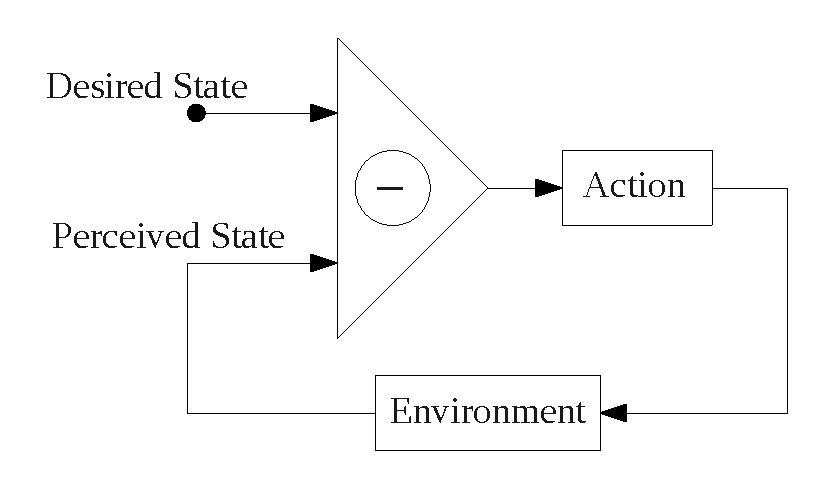
\includegraphics[width=6cm]{gfx/feedback_control}
  \caption[The feedback control model for accomplishing a single goal]{The feedback control model for accomplishing a single goal.}
  \label{fig:feedback_control}
\end{figure}

Now that we have discussed the basic model of learning from experience
what good goal states may be from rewards, let us consider the
representations for the state space of the perceptions and actions of
our model.  Control theory has given us many useful models for agents
that control continuous environments.  For example,
Figure~\ref{fig:feedback_control} shows a simple difference feedback
control circuit that is used in simple linear control systems.  The
system is given a desired state, there is a difference device that
calculates the difference between the actual perceived value from the
environment, and the control system then executes an action based on
that difference, which affects the environment.  The result in such a
negative feedback loop is that the agent's perception of the
environment is closer to the desired state.

\section{Means-End Analysis}

In 1959, Newell, Shaw, and Simon published a report on a means-end
analysis model that was designed to solve any symbolically represented
problem \citep{newell:1959}.  Their system was called the \ac{GPS},
and worked by being able to work with relational representations of
current and desired states.  The agent had a catalogue of differences
between states that it knew how to minimize.  The system worked by
finding the largest difference and executing the associated method for
reducing this difference.  This work has grown into the Soar model
\citep{newell:1990} for better solving symbolic planning problems, and
dealing with impasses for when the planning search runs out of
options.

\section{Difference-Engine Model for Accomplishing Multiple Goals}

\begin{figure}[bth]
  \center
  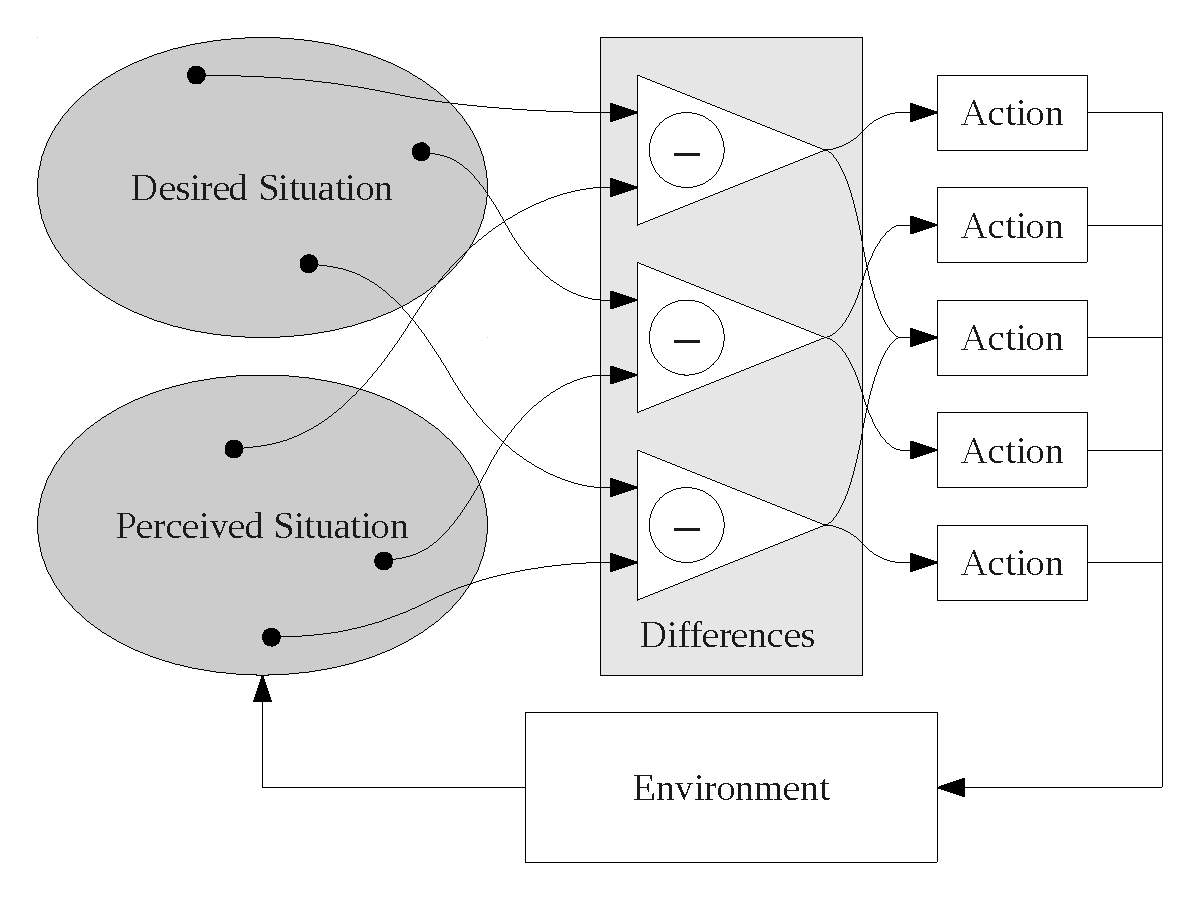
\includegraphics[height=6cm]{gfx/difference_engine_feedback_control}
  \caption[The difference engine model for accomplishing multiple goals]{The difference engine model for accomplishing multiple goals.}
  \label{fig:difference_engine_feedback_control}
\end{figure}

\citep[p.~78]{minsky:1988}






